\section{Introduction}

\begin{wrapfigure}{r}{0.5\textwidth}
  \begin{center}
    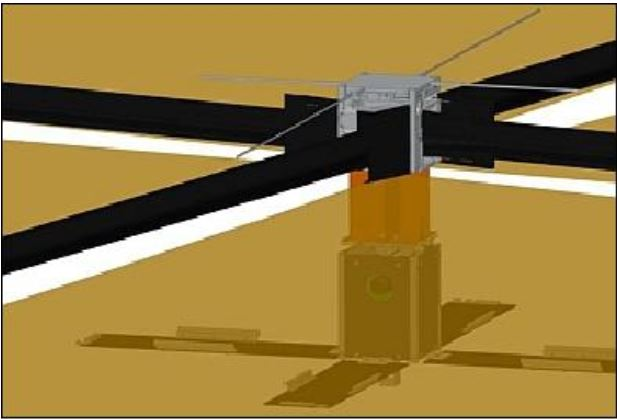
\includegraphics[width=0.5\textwidth]{images/satellitesail.JPG}\\
  \end{center}
  \caption{Deployable booms attached to the solar sails used in DeOrbitSail from source \cite{ESA}}
  \label{fig:sail}
\end{wrapfigure}

The market for small satellites has been growing due to their fast development times, relative low cost of development, compatibility to launch with multiple launchers and the capability to deploy in multiple constellations. However the ever increasing mission requirements often are in contradiction to the mass and volume constraints which are subject to the satellite. Many systems such as solar panels, telescopes, solar sails etc. are in need of reliable deployment of structural booms and arrays for power generation, communications and scientific systems and deployable structures are a solution to that problem. Deployable structures like the one shown in figure \ref{fig:a12} can change their shape and size from a compact configuration to a large, open configuration. 
\begin{wrapfigure}{l}{0.45\textwidth}
  \begin{center}
    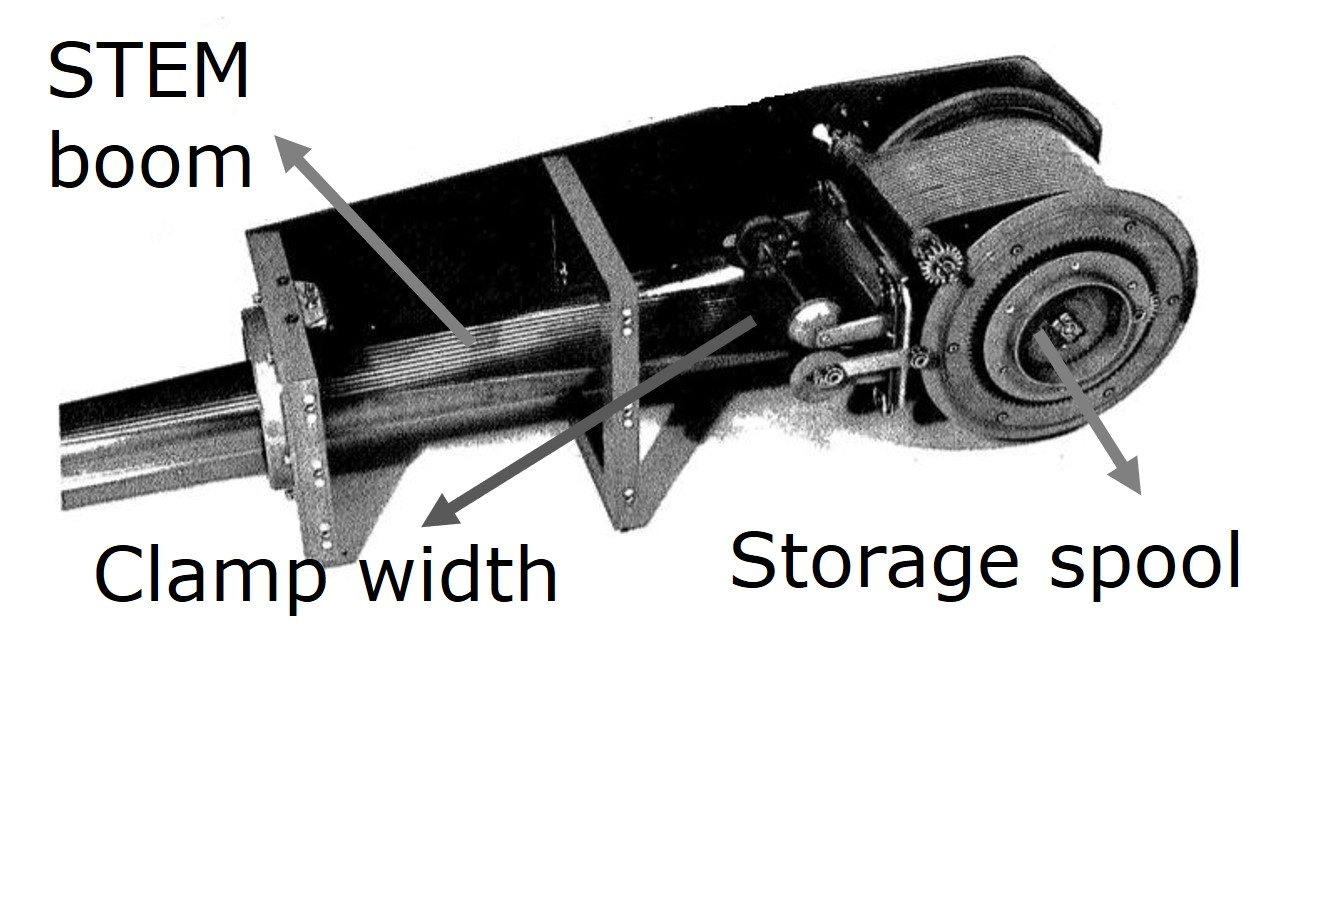
\includegraphics[width=0.45\textwidth]{images/deployerboom.jpg}
  \end{center}
  \caption{A-12 deployer for STEM boom used in apollo missions \cite{NASA}}
  \label{fig:a12}
\end{wrapfigure}
Using the example of the DeOrbit sail satellite developed by the European Space Agency (ESA) \cite{ESA}, deployable booms support a sail in the deorbiting phase of the mission. In the de-orbit stage, compressive loading would be applied to the tip of the boom by the sail due to force of the atmosphere on the sail. However, this can lead to buckling of the boom after surpassing its limit, in which case the sail would fail. Thus, accurate estimates of this limit is vital for the technology to be used. This can be achieved using finite element analysis (FEA) in which the conditions found in space can be replicated. To ensure accurate modelling of the problem in FEA, the boundary conditions of the boom at the root should be modelled accurately. The booms are attached to a satellite deployer shown in figure \ref{fig:a12} using screws spaced apart which ensure that the boom can roll up on the spool. This ensures the deployment of the boom in an aligned and controlled manner. However, in FEA simulations across literature, predominantly an encastered root condition has been applied at the root which can lead to differences in the properties of the boom, since in the actual application the boom would likely be flattened at the end to an extent as can be seen clearly in figure \ref{fig:a12}. 

Thus the aim of this project is to compare the effects on the bending stiffness and the maximum reaction moment of a boom with varying widths of the attachment screws. This is implemented using an analytical model developed and analysed in ABAQUS FEA software \cite{ABAQUS}.     

The literature review in section \ref{sec:litreview} gives an overview of deployable structures, computational models and tape spring behaviour. The methodology in section \ref{sec:method} describes the development of the FEA model of the boom. Results and discussions in section \ref{sec:results} analyses the plots of the lateral displacement, reaction moment, bending stiffness and ploy length. Finally the conclusion in section \ref{sec:conclusion} outlines the future work possibilities of the project. 

\newpage